\section{A Long List of Lemmas}
From this point forward in the section we assume that \(\DConf_n(\Gamma)\) is an \(m\)-manifold without boundary
and \(M\) is an \((m-1)\)-matching in \(\Gamma\).

\subsection{Minimum Graph Size and Key Lemma}

\begin{lem}
\label{lem:graph-size}
    \(\Gamma\) has at least \(m + n\) vertices and \(n \ge m\).
\end{lem}

\begin{proof}
    If \(\Gamma\) has less than \(n\) vertices, then \(\DConf_n(\Gamma)\) is empty;
    so, suppose \(\Gamma\) has at least \(n\) vertices.
    If \(\Gamma\) has less than \(n + m\) vertices, then
    for any configuration of \(n\) particles on \(\Gamma\)
    at most \(m-1\) particles can simultaneously move.
    Since exactly \(m\) particles need to be able to simultaneously move for an \(m\)-cube 
    to exist in \(\DConf_n(\Gamma)\), no configuration in \(\DConf_n(\Gamma)\)
    can have a neighborhood homeomorphic to an open set in \(\mathbb{R}^m\).

    Similarly, if \(n < m\), then there are not enough particles that can simultaneously move
    for an \(m\)-cube to exist in \(\DConf_n(\Gamma)\). So, \(n \ge m\). 
\end{proof}

\begin{rem}
\(\Gamma - V(M)\) then has at least \(m + n - 2(m - 1) = n - m + 2 = n - (m - 1) + 1\) vertices.
\end{rem}

This next lemma is the key to all following proofs.
The idea is that if we have an \((m-1)\)-cube in the configuration space,
then there needs to be exactly two \(m\)-cubes that border it for the points
in that \((m-1)\)-cube to look locally like \(\mathbb{R}^m\).

\begin{lem}
    \label{lem:special-edges}
    For any collection \(\mathcal{V}\) of \(n - (m - 1)\) vertices in \(\Gamma - V(M)\), there exists exactly \textbf{two}
    edges \(e_1\) and \(e_2\) in \(\Gamma - V(M)\) that are incident to vertices in \(\mathcal{V}\)
    and vertices not in \(\mathcal{V}\).

    Furthermore, these edges \(e_1\) and \(e_2\) satisfy all of the following conditions.
    \begin{enumerate}[label=(\roman*)]
    \item \(e_1\) and \(e_2\) are both incident to one vertex in \(\mathcal{V}\)
    \item \(e_1\) and \(e_2\) are both incident to one vertex not in \(\mathcal{V}\)
    \item \(e_1\) and \(e_2\) share exactly one common vertex.
    \end{enumerate}

    Equivalently, exactly one of the following hold in Figure \ref{fig:lem:special-edges}
    \begin{figure}[h!]
        \centering
        \begin{enumerate*}[label=(\arabic*)]
            \item \label{fig:lem:manifolds_1_1}
            \begin{minipage}{.3\textwidth}
                \centering
                \(v_1 \in \mathcal{V}\) \textit{and} \(w_1, w_2 \not \in \mathcal{V}\) \\
                \vspace{1em}
                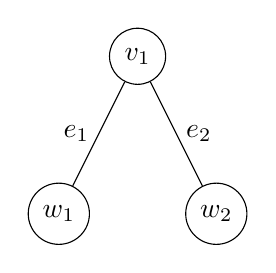
\begin{tikzpicture}
                    \node (v1) at (3, 2) [circle, draw] {\(v_1\)};
                    \node (w1) at (2, 0) [circle, draw] {\(w_1\)};
                    \node (w2) at (4, 0) [circle, draw] {\(w_2\)};

                    \draw (v1) -- (w1) node[midway, left] {\(e_1\)};
                    \draw (v1) -- (w2) node[midway, right] {\(e_2\)};
                \end{tikzpicture} 
            \end{minipage}

            \hspace{3em}

            \item \label{fig:lem:manifolds_1_2}
            \begin{minipage}{.3\textwidth}
                \centering
                \(v_1, v_2 \in \mathcal{V}\) \textit{and} \(w_1 \not \in \mathcal{V}\) \\
                \vspace{1em}
                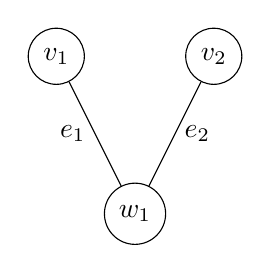
\begin{tikzpicture}
                    \node (v1) at (2, 2) [circle, draw] {\(v_1\)};
                    \node (v2) at (4, 2) [circle, draw] {\(v_2\)};
                    \node (w1) at (3, 0) [circle, draw] {\(w_1\)};

                    \draw (v1) -- (w1) node[midway, left] {\(e_1\)};
                    \draw (v2) -- (w1) node[midway, right] {\(e_2\)};
                \end{tikzpicture}
            \end{minipage}
        \end{enumerate*}
        \caption{Lemma \ref{lem:special-edges} possibilities.}
        \label{fig:lem:special-edges}
    \end{figure}
\end{lem}

\begin{proof}
    Let \(\mathcal{V}\) be a collection of \(n - (m - 1)\) vertices in \(\Gamma - V(M)\)
    and \(p\) be the configuration of \(n\) particles placed on \(\Gamma\) such that
    \(n - (m - 1)\) particles are placed at each vertex in \(\mathcal{V}\)
    and \(m - 1\) particles on each edge in \(M\).
    
    As the particles move move along the edges in \(M\), an \((m-1)\)-cube containing \(p\)
    is spanned in \(\DConf_n(\Gamma)\).
    Since the configuration space is an \(m\)-manifold without boundary, 
    this \((m-1)\)-cube must border exactly two distinct \(m\)-cubes.
    For this \((m-1)\)-cube to border two \(m\)-cubes,
    there needs to exist \textbf{two} additional mutually exclusive particle movements.
    Let \(v_1, v_2 \in \mathcal{V}\) and \(w_1, w_2 \not \in \mathcal{V}\) be the vertices corresponding
    to the origins and destinations of these additional particle movements.
    If \(v_1 \neq v_2\) and \(w_1 \neq w_2\), then two particles would be able to move simultaneously
    resulting in an \((m+1)\)-cube being spanned in \(\DConf_n(\Gamma)\) contradicting 
    that it is an \(m\)-manifold.
\end{proof}

This lemma is extremely powerful as the next lemma illustrates.

\begin{lem}
    \label{lem:manifold-max-degree}
    Every vertex in \(\Gamma - V(M)\) has degree at most \(3\).
\end{lem}

\begin{proof}
    Suppose \(\Gamma - V(M)\) has a vertex \(v\) with degree greater than \(3\).
    We proceed by cases on \(n\).

    \textbf{Case 1:} \(n \le m - 1 + \deg(v)\)
    In the context of Lemma \ref{lem:special-edges},
    construct \(\mathcal{V}\) so that all \(n - (m - 1) = n - m + 1\)
    vertices are on the vertices adjacent to \(v\).
    Then, there are too many edges with one endpoint in \(\mathcal{V}\)
    and other outside of \(\mathcal{V}\) for Lemma \ref{lem:special-edges} to hold.

    \textbf{Case 2:} \(n > m - 1 + \deg(v)\)
    Lemma \ref{lem:graph-size} guarantees that \(\Gamma - V(M)\) has at least
    \(n + m - 2(m - 1) = n - m + 2\) vertices.
    So, \(\abs{V(\Gamma - V(M))} > \deg(v) + 1\).
    More importantly, it's clear now that we can now construct a \(\mathcal{V}\)
    so that it contains \(v\) and every vertex adjacent to \(v\).
    By Lemma \ref{lem:special-edges}, there is at least one vertex \(w \not \in \mathcal{V}\).
    Let \(\mathcal{V}' = \left(\mathcal{V}\setminus\{v\}\right)\cup\{w\}\) i.e. 
    swap out \(v\) for \(w\) in \(\mathcal{V}\).
    Then, again there are now too many edges with one endpoint in \(\mathcal{V}'\)
    and another outside of \(\mathcal{V}'\) to for Lemma \ref{lem:special-edges} to hold.
\end{proof}

\subsection{\(m = 1\) or No Cycles}

\begin{lem}
    \label{lem:manifold-is-claw}
    If \(\Gamma - V(M)\) contains a degree \(3\) vertex,
    then \(\Gamma - V(M) \cong K_{1,3}\) and \(n = m + 1\).
\end{lem}

\begin{proof}
    Suppose \(\Gamma - V(M)\) contains a degree \(3\) vertex \(v\).
    First we show that \(n\) must be equal to \(m + 1\) by considering two cases.

    \textbf{Case 1:} \(n > m + 1\)
    % TODO Clean up
    Fill up the \(Y\)-graph.
    There must be at least one free vertex.
    Put a particle there instead of at \(v\)
    Book.

    \textbf{Case 2:} \(n < m + 1\)
    In this case \(n\) must equal \(m\) by Lemma \ref{lem:graph-size}.
    Let \(\mathcal{V}\) consist of just the vertex \(v\).
    Then, there are too many edges with one endpoint in \(\mathcal{V}\)
    and another outside of \(\mathcal{V}\) to for Lemma \ref{lem:special-edges} to hold.
    Namely, the three edges incident to \(v\).

    Now we show that there cannot be any other vertices in \(\Gamma - V(M)\) besides \(v\) and its neighbors.
    Suppose there was a vertex \(w \neq v\) in \(\Gamma - V(M)\) that is not adjacent to \(v\).
    Let \(\mathcal{V} = \{v, w\}\).
    Then, again there are too many edges with one endpoint in \(\mathcal{V}\)
    and another outside of \(\mathcal{V}\) to for Lemma \ref{lem:special-edges} to hold.
    Namely, the three edges incident to \(v\).

    Finally, we show that there cannot be any edges in \(\Gamma - V(M)\)
    besides the three edges incident to \(v\).

    Suppose there was another edge \(e\) in \(\Gamma - V(M)\) not incident to \(v\) and
    let \(a\) and \(b\) be the vertices incident to \(e\) and \(c\) be the other vertex adjacent to \(v\)
    (see Figure \ref{fig:lem:manifold-is-claw:1}).

    \begin{figure}
        \centering
        \begin{tikzpicture}
            \node (v) at (0,0) [circle, draw] {\(v\)};
            \node (a) at (-2,-2) [circle, draw] {\(a\)};
            \node (b) at (2,-2) [circle, draw] {\(b\)};
            \node (c) at (0,2) [circle, draw] {\(c\)};

            \draw (v) -- (a);
            \draw (v) -- (b);
            \draw (v) -- (c);
            \draw (a) -- (b) node[midway, below] {\(e\)};
        \end{tikzpicture}
        \caption{\(\Gamma - V(M)\) with an extra edge \(e\)}
        \label{fig:lem:manifold-is-claw:1}
    \end{figure}

    Let \(\mathcal{V} = \{a, c\}\).
    Then, again there are too many edges with one endpoint in \(\mathcal{V}\) and another outside of \(\mathcal{V}\).
    Namely, \(cv\), \(av\), and \(bv\).

    Therefore \(\Gamma - V(M)\) must consist solely of \(v\), its neighbors, and the edges incident to \(v\).
\end{proof}

\begin{lem}
    If \(m = 1\), then \(\Gamma \cong K_{1,3}\) and \(n = 2\),
    or \(\Gamma\) is one or more cycles and \(n \in \{1, \abs{V(\Gamma)} - 1\}\) 
\end{lem}

\begin{proof}
    It is sufficient to show that the degree of every vertex in \(\Gamma\) is exactly \(2\).
    Let \(v\) be some vertex in \(\Gamma\). By Lemma \ref{lem:graph-size}, there exists \(n\) other vertices in \(\Gamma\).
    The edges \(e_1\) and \(e_2\) guaranteed by Lemma \ref{lem:special-edges} must then both be incident to \(v\)
    and there can be no other edges incident to \(v\) and these \(n\) vertices.
    If there were another edge incident to \(v\), then \(v\) would have degree at least \(3\)
    meaning \(\Gamma\) would have to be \(K_{1,3}\).
    So, then \(n = 2\) and \(\Gamma\) is just \(K_{1,3}\).

    Otherwise, \(v\) has degree exactly \(2\).
    Since \(v\) was arbitrary, every vertex in \(\Gamma\) has degree exactly \(2\)
    meaning, \(\Gamma\) is one or more cycles.
    If \(1 < n < \abs{V(\Gamma)} - 1\), then there are too many ways for particles to move.
\end{proof}

Now that the \(m = 1\) case is completely determined, we only consider when \(m \ge 2\) from this point onward.

\begin{lem}
    \(\Gamma - V(M)\) must be \(K_{1,3}\) or contain a cycle.
\end{lem}

\begin{proof}
    % TODO rephrase as to not use particle placement language
    Suppose that \(\Gamma - V(M)\) contains no vertices of degree 3 nor any cycles.
    Then \(\Gamma - V(M)\) is a forest whose trees are paths.
    Since \(\Gamma - V(M)\) has at least \(m + n - 2(m - 1) = n - m + 2\) vertices by Lemma \ref{lem:graph-size},
    we can place \(n - (m - 1)\) particles filling up the paths.
    Then there is only one edge contradicting Lemma \ref{lem:special-edges}.
\end{proof}

\subsection{\(m > 1\) and Cycles}
Since we know what happens when \(m = 1\) or \(\Gamma - V(M)\) contains no cycles.
Continue to assume that \(m > 1\) but now also suppose \(\Gamma - V(M)\) contains a cycle \(C\).

\begin{lem}
\label{lem:manifold-one-cycle}
    \(\Gamma - V(M)\) contains at most one cycle.
\end{lem}

\begin{proof}
    Suppose \(\Gamma - V(M)\) contains another cycle \(D\) distinct from \(C\).
    Since \(m > 1\), \(M\) contains at least one edge \(e\).
    Let \(v_1\) be some vertex on \(C\) and \(w_1\) be adjacent to \(v_1\) on \(C\).
    Also, let \(v_2\) be some vertex on \(D\) and \(w_2\) be adjacent to \(v_2\) on \(D\).

    Define \(M' = (M \setminus \{e\}) \cup \{v_1 w_1\}\) and \(M'' = (M \setminus \{e\}) \cup \{v_2 w_2\}\).
    Initially we showed that \(\Gamma - V(M)\) is a disjoint union of cycles.
    This fact does not depend on which matching we chose.
    Therefore \(\Gamma - V(M')\) is also a disjoint union of cycles.
    So, \(e\) must belong to a cycle in \(\Gamma - V(M')\).
    The only way for this to happen is if \(e\) belongs to the ``broken cycle'' \(C - V(\{v_1 w_1\})\)
    in \(\Gamma - V(M')\).
    But then, \(v_1\) has degree \(3\) in \(\Gamma - V(M'')\) if \(C\) has length greater than \(3\)
    or degree \(4\) if \(C\) has length equal to \(3\).
    Lemma \ref{lem:manifold-max-degree} forces \(C\) to have length greater than \(3\)
    and Lemma \ref{lem:manifold-is-claw} requires that \(\Gamma - V(M'')\) is just \(v_1\) and its neighbors.
    However, \(V - V(M'')\) has at least \(6\) vertices:
    the vertices incident to \(e\), the vertices on \(C\), and the vertices on \(D - V(\{v_2 w_2\})\).
\end{proof}

\begin{lem}
    \label{lem:manifold-cycle-equality}
    If \(n = m\) or \(\Gamma - V(M)\) has \(n - (m - 1) + 1\) vertices, then \(\Gamma - V(M) \cong C\).
\end{lem}

\begin{proof}
    First, suppose \(n = m\) and let \(v\) be some vertex in \(\Gamma - V(M)\).
    Since \(m = n\), any collection of \(n - (m - 1)\) vertices in \(\Gamma - V(M)\)
    is just a single vertex. Define \(\mathcal{V} = \{v\}\) 
    Then, Lemma \ref{lem:special-edges} guarantees that there are exactly two edges
    incident to \(v\). Since \(v\) was arbitrary, every vertex in \(\Gamma - V(M)\)
    has degree \(2\).

    Similarly, if \(\Gamma - V(M)\) has \(n - (m - 1) + 1\) vertices,
    then any collection of \(n - (m - 1)\) vertices in \(\Gamma - V(M)\)
    will be missing exactly one vertex in \(\Gamma - V(M)\).
    So, if \(v\) is any vertex in \(\Gamma - V(M)\),
    define \(\mathcal{V}\) to just be all of \(\Gamma - V(M)\) except for \(v\).
    Then, Lemma \ref{lem:special-edges} guarantees that there are exactly two edges
    incident to \(v\) and since \(v\) was arbitrary, every vertex in \(\Gamma - V(M)\)
    has degree \(2\).

    Therefore, in either case every vertex in \(\Gamma - V(M)\) has degree \(2\)
    meaning \(\Gamma - V(M)\) is a collection of cycles.
    However, Lemma \ref{lem:manifold-one-cycle} guarantees that this cycle is just \(C\).
\end{proof}

\begin{lem}
    \label{lem:manifold-cycle-length-1}
    \(C\) has length at most \(4\).
\end{lem}

\begin{proof}
    Suppose \(C\) has length greater than \(4\) and let \(v_1, \cdots, v_5\) be \(5\) consecutive vertices on \(C\).
    First we show that there cannot be more than \(n - (m - 1) + 1\) vertices in \(\Gamma - V(M)\).
    Suppose this were so and let \(\mathcal{V}\) be any collection of \(n - (m - 1)\) vertices in \(\Gamma - V(M)\)
    containing \(v_1\) and \(v_4\) but not \(v_2\) and \(v_3\).
    Then, the edges \(v_1 v_2\) and \(v_3 v_4\) are incident to one vertex in \(\mathcal{V}\)
    and one vertex outside of \(\mathcal{V}\) but
    do not share a common vertex contradicting Lemma \ref{lem:special-edges}.
    Hence \(\Gamma - V(M)\) contains at most \(n - (m - 1) + 1\) vertices.
    Moreover, Lemma \ref{lem:graph-size} guarantees that \(\Gamma - V(M)\) has at
    least \(n + m - 2(m - 1) = n - (m - 1) + 1\) vertices. 
    So, \(\Gamma - V(M)\) must have exactly \(n - (m - 1) + 1\) vertices.

    % The above argument only relies on the fact that C has more than 3 vertices.

    Lemma \ref{lem:manifold-cycle-equality} then guarantees that every vertex in \(\Gamma - V(M)\) has degree \(2\).
    Since \(m > 1\), \(M\) contains at least one edge \(e\). Let \(w_1\) and \(w_2\) be the vertices incident to \(e\).
    Define \(M' = (M \setminus \{e\}) \cup \{v_2 v_3\}\).
    The fact that every vertex in \(\Gamma - V(M)\) has degree \(2\)
    does not depend on which matching we choose. So, every vertex in \(\Gamma - V(M')\) also must have degree \(2\).
    So, \(w_1\) and \(w_2\) must be adjacent to \(v_1\) or \(v_4\) in \(\Gamma - V(M')\) since those vertices
    are the only vertices in \(\Gamma - V(M')\) that could have degree less than \(2\).

    Without a loss of generality suppose \(w_1\) is adjacent to \(v_4\) in \(\Gamma - V(M')\) (see Figure \ref{fig:lem:manifold-cycle-length-1:1})

    \begin{figure}[h!]
        \centering
        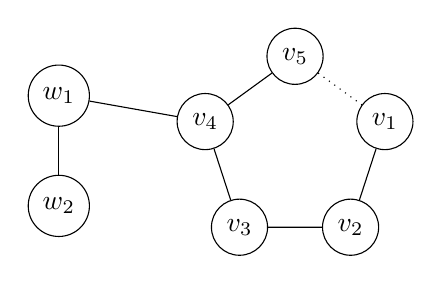
\begin{tikzpicture}
            \foreach \i in {1,...,5} \node (v\i) at ({90-72*\i}:1.2) [circle, draw] {\(v_{\i}\)};
            \draw (v1) -- (v2) -- (v3) -- (v4) -- (v5);

            \draw[dotted] (v5) -- (v1);

            \node (w1) at (-3,.7) [circle, draw] {\(w_1\)};
            \node (w2) at (-3,-.7) [circle, draw] {\(w_2\)};
            \draw (w1) -- (w2);

            \draw (w1) -- (v4);
        \end{tikzpicture}
        \caption{\(w_1\) is adjacent to \(v_4\) in \(\Gamma - V(M')\)}
        \label{fig:lem:manifold-cycle-length-1:1}
    \end{figure}

    Now, define \(M'' = (M \setminus \{e\}) \cup \{v_1 v_2\}\).
    Then, \(v_4\) has degree \(3\) in \(\Gamma - V(M'')\).
    Lemma \ref{lem:manifold-is-claw} then requires that \(\Gamma - V(M'')\) is just \(v_4\) and its neighbors.
    However, \(\Gamma - V(M'')\) has at least \(5\) vertices.
\end{proof}

\begin{lem}
    \label{lem:manifold-cycle-length-2}
    \(\Gamma - V(M)\) has at most \(4\) vertices.
\end{lem}

\begin{proof}
    It follows from Lemma \ref{lem:manifold-cycle-equality} and 
    Lemma \ref{lem:manifold-cycle-length-1}
    that if \(n = m\) or \(\Gamma - V(M)\) has \(n - (m - 1) + 1\), then \(\Gamma - V(M)\) has at most \(4\) vertices.
    So, suppose \(n > m\) and that \(\Gamma - V(M)\) has more than \(\max\{4, n - (m - 1) + 1\}\) vertices.
    % Taking the max here is fine since graph size lemma guarantees \Gamma - V(M) has at least n - (m - 1) + 1 vertices.
    We proceed by cases on the length of \(C\).

    \textbf{Case 1:} \(C\) has length \(3\).
    In this case there must be at least two other vertices in \(\Gamma - V(M)\)
    other than the three vertices on \(C\).
    Let \(v_1, v_2, v_3\) be the vertices on \(C\) and \(\mathcal{V}\)
    be a collection of \(n - (m - 1)\) vertices containing \(v_1\), \(v_2\), and \(v_3\).

    Lemma \ref{lem:special-edges} then guarantees that there are exactly two edges: \(e_1\) and \(e_2\)
    with one endpoint in \(\mathcal{V}\) and another outside of \(\mathcal{V}\)
    which share a common vertex.

    Notice that neither \(e_1\) nor \(e_2\) can be incident vertices on \(C\)
    otherwise we would have a degree \(4\) or \(3\) vertex contradicting 
    Lemma \ref{lem:manifold-max-degree} or Lemma \ref{lem:manifold-is-claw} respectively.
    Hence we have one of two cases: \(e_1\) and \(e_2\) share a common vertex in \(\mathcal{V}\)
    or \(e_1\) and \(e_2\) share a common vertex outside of \(\mathcal{V}\).

    \textbf{Subcase 1:} \(e_1\) and \(e_2\) share a common vertex in \(\mathcal{V}\).
    Let \(v_4\) be this common vertex and \(w_1\) and \(w_2\) be the other endpoints of \(e_1\) and \(e_2\) respectively (see Figure \ref{fig:lem:manifold-cycle-length-2:1}).

    \begin{figure}[h!]
        \centering
        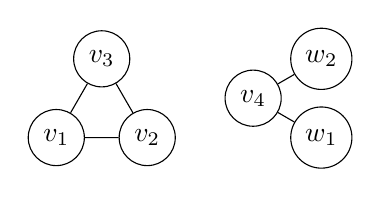
\begin{tikzpicture}
            \node (v1) at (0,0) [circle, draw] {\(v_1\)};
            \node (v2) at (1.155,0) [circle, draw] {\(v_2\)};
            \node (v3) at (0.577,1) [circle, draw] {\(v_3\)};
            \draw (v1) -- (v2) -- (v3) -- (v1);

            \node (v4) at (2.5, .5) [circle, draw] {\(v_4\)};
            \node (w1) at (3.366, 0) [circle, draw] {\(w_1\)};
            \node (w2) at (3.366, 1) [circle, draw] {\(w_2\)};
            \draw (w2) -- (v4) -- (w1);
        \end{tikzpicture}
        \caption{\(e_1\) and \(e_2\) share a common vertex in \(\mathcal{V}\)}
        \label{fig:lem:manifold-cycle-length-2:1}
    \end{figure}

    Let \(\mathcal{V}' = (\mathcal{V} \setminus \{v_1\}) \cup \{w_1\}\).
    Then, there are now three edges with one endpoint in \(\mathcal{V}'\)
    and another outside of \(\mathcal{V}'\) contradicting Lemma \ref{lem:special-edges}.
    Namely, the edges \(e_2 = v_4 w_2\), \(v_1 v_2\), and \(v_1 v_3\).


    \textbf{Subcase 2:} \(e_1\) and \(e_2\) share common vertex outside of \(\mathcal{V}\).
    Let \(w_1\) be this common vertex and \(v_4\) and \(v_5\) be the other endpoints of \(e_1\) and \(e_2\) respectively (see Figure \ref{fig:lem:manifold-cycle-length-2:2}).

    \begin{figure}[h!]
        \centering
        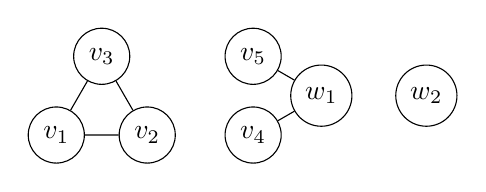
\begin{tikzpicture}
            \node (v1) at (0,0) [circle, draw] {\(v_1\)};
            \node (v2) at (1.155,0) [circle, draw] {\(v_2\)};
            \node (v3) at (0.577,1) [circle, draw] {\(v_3\)};
            \draw (v1) -- (v2) -- (v3) -- (v1);

            \node (v4) at (2.5, 0) [circle, draw] {\(v_4\)};
            \node (v5) at (2.5, 1) [circle, draw] {\(v_5\)};
            \node (w1) at (3.366, 0.5) [circle, draw] {\(w_1\)};
            \draw (v4) -- (w1) -- (v5);

            \node (w2) at (4.7, 0.5) [circle, draw] {\(w_2\)};
        \end{tikzpicture}
        \caption{\(e_1\) and \(e_2\) share a common vertex outside of \(\mathcal{V}\)}
        \label{fig:lem:manifold-cycle-length-2:2}
    \end{figure}

    Since \(\Gamma - V(M)\) has more than \(n - (m - 1) + 1\) vertices, there must be at least one other vertex \(w_2\)
    outside of \(\mathcal{V}\) besides \(w_1\). 
    Let \(\mathcal{V}'' = (\mathcal{V} \setminus \{v_1\}) \cup \{w_2\}\).
    The edges \(e_1 = v_4 w_1\), \(e_2 = v_5 w_1\), \(v_1 v_2\), and \(v_1 v_3\)
    all have one endpoint in \(\mathcal{V}''\) and another outside of \(\mathcal{V}''\)
    contradicting Lemma \ref{lem:special-edges}.


    \textbf{Case 2:} \(C\) has length \(4\).
    Let \(v_1\), \(v_2\), \(v_3\), and \(v_4\) be the vertices on \(C\) (see Figure \ref{fig:lem:manifold-cycle-length-2:3}).
    Since \(\Gamma - V(M)\) has more than \(\max\{4, n - (m - 1) + 1\}\) vertices,
    for any collection of \(n - (m - 1)\) vertices in \(\Gamma - V(M)\),
    there will have at least two other vertices in \(\Gamma - V(M)\).

    Let \(\mathcal{V}\) consist of \(n - (m - 1)\) vertices other than \(v_1\) and \(v_3\).
    Then, the edges \(v_1 v_2\), \(v_1, v_4\), \(v_3 v_2\), and \(v_3 v_4\)
    all have one endpoint in \(\mathcal{V}\) and another outside of \(\mathcal{V}\)
    contradicting Lemma \ref{lem:special-edges}

    \begin{figure}[h!]
        \centering
        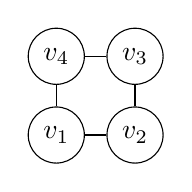
\begin{tikzpicture}
            \node (v1) at (0, 0) [circle, draw] {\(v_1\)};
            \node (v2) at (1, 0) [circle, draw] {\(v_2\)};
            \node (v3) at (1, 1) [circle, draw] {\(v_3\)};
            \node (v4) at (0, 1) [circle, draw] {\(v_4\)};
            \draw (v1) -- (v2) -- (v3) -- (v4) -- (v1);
        \end{tikzpicture}
        \caption{Cycle \(C\) of length \(4\)}
        \label{fig:lem:manifold-cycle-length-2:3}
    \end{figure}


    \textbf{Case 3:} \(C\) has length greater than \(4\).
    This case is handled by Lemma \ref{lem:manifold-cycle-length-1}.
\end{proof}

\begin{lem}
    If \(C\) has length \(3\), then exactly one of the following hold.
    \begin{enumerate}[label=(\roman*)]
        \item \(\Gamma - V(M) \cong K_3\) and \(n = m\) or \(n = m + 1\)
        \item \(\Gamma - V(M) \cong K_3 \cup K_1\) and \(n = m + 1\)
    \end{enumerate}
\end{lem}
\begin{proof}
    Suppose \(C\) has length \(3\). Then, \(C \cong K_3\).
    Lemma \ref{lem:manifold-cycle-length-2} then guarantees that \(\Gamma - V(M)\) is \(K_3\)
    or has \(K_3 \cup K_1\) as a subgraph.

    \textbf{Case 1:} \(\Gamma - V(M) \cong K_3\).
    Notice that \(\Gamma\) must have \(2m + 1\) vertices.
    Lemma \ref{lem:graph-size} then guarantees that \(m \le n \le m + 1\).

    \textbf{Case 2:} \(\Gamma - V(M)\) has \(K_3 \cup K_1\) as a subgraph.
    The isolated vertex in \(\Gamma - V(M)\) cannot connect to any other vertices otherwise
    we would have a degree \(3\) vertex in \(\Gamma - V(M)\).
    However, Lemma \ref{lem:manifold-is-claw} would imply that \(\Gamma - V(M)\) is just this vertex and its neighbors
    contradicting that \(\Gamma - V(M)\) contains \(K_3\) as a subgraph.
    So, \(\Gamma - V(M) \cong K_3 \cup K_1\).

    Similar to before, since \(\Gamma - V(M)\) has exactly \(4\) vertices,
    \(\Gamma\) must have exactly \(2m + 2\) vertices.
    Lemma \ref{lem:graph-size} then guarantees that \(m \le n \le m + 2\).
    Lemma \ref{lem:manifold-cycle-equality} prevents \(n = m\).
    Also, since \(\Gamma - V(M)\) has \(4\) vertices, if \(n = m + 2\)   
    then \(4 = n - (m - 1) + 1\) contradicting Lemma \ref{lem:manifold-cycle-equality}.

\end{proof}

\begin{lem}
    If \(C\) does not have length \(3\), then \(\Gamma - V(M) \cong K_{2,2}\) and \(n = m\) or \(n = m + 2\).
\end{lem}

\begin{proof}
    If \(C\) does not have length \(3\), then Lemma \ref{lem:manifold-cycle-length-1} guarantees that \(C\) has length \(4\).
    Lemma \ref{lem:manifold-cycle-length-2} then guarantees that \(\Gamma - V(M)\) is just \(C\).
    Since \(4\)-cycles are isomorphic to \(K_{2,2}\), it follows that \(\Gamma - V(M) \cong K_{2,2}\).

    Since \(\Gamma - V(M)\) has exactly \(4\) vertices, \(\Gamma\) itself has exactly \(2m + 2\) vertices.
    Lemma \ref{lem:graph-size} then guarantees that \(m \le n \le m + 2\).
    Suppose \(n = m + 1\) and let \(\mathcal{V}\) consist of two non-adjacent vertices on \(C\).
    Then, there are too many edges with one endpoint in \(\mathcal{V}\)
    and another outside of \(\mathcal{V}\) for Lemma \ref{lem:special-edges} to hold.
\end{proof}